
\section{Abbildungen/Funktionen}

\textbf{Abbildung:} Definitionsbereich, Wertebereich, Bild, Urbild, Einschränkung\\
\textbf{Definition (Abbildung):}\\
Seien $\mathbb{A},\mathbb{B}$ Mengen, dann gilt:\\
Eine Abbildung $f$ von $\mathbb{A}$ nach $\mathbb{B}$ ist eine Vorschrift, die jeden $x\in\mathbb{A}$ genau ein Element $y=f(x)\in\mathbb{B}$ zuweist.\\
\begin{align*}
	f:\mathbb{A}\rightarrow \mathbb{B}\qquad x\rightarrow f(x)
\end{align*}
Die Menge $ \mathbb{A}$ entspricht den Definitionsbereich $\mathbb{D}$.\\
Die Menge $ \mathbb{B}$ entspricht den Wertebereich $\mathbb{W}$.\vspace*{2mm}\\
Man spricht von einer Funktion, wenn gilt:\\
\begin{align*}
	\mathbb{A},\mathbb{B}\subset \mathbb{R}\Rightarrow f:\mathbb{A}\rightarrow \mathbb{B}\\
\end{align*}
Beispiel:\\
\textbullet $\qquad f_1:\mathbb{R}\rightarrow \mathbb{R}\text{ ,  }  x\rightarrow 2x $\vspace*{2mm}\\
\begin{center}
	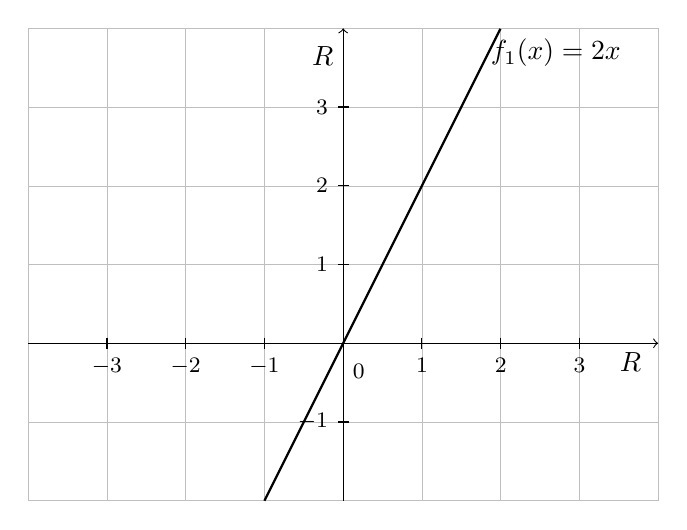
\begin{tikzpicture}
		
		% Gitternetzlinien
		\draw[xstep=1cm, ystep=1cm, very thin, color=lightgray] (-4,4) grid (4,-2);
		% x-Achse
		\draw[->] (-4,0) -- (4,0) node[below,xshift=-1em] {$\mathbb{R}$}; 
		%Zahlen auf x-Achse
		\foreach \x in {-3,...,-1}
		\draw[shift={(\x,0)},color=black] (0pt,2pt) -- (0pt,-2pt) node[below] {\footnotesize $\x$};
		\foreach \x in {1,...,3}
		\draw[shift={(\x,0)},color=black] (0pt,2pt) -- (0pt,-2pt) node[below] {\footnotesize $\x$};
		% y-Achse 
		\draw[->] (0,-2) -- (0,4) node[left,yshift=-1em] {$\mathbb{R}$};%node[above left]
		%Zahlen auf y-Achse
		\foreach \y in {-1,...,-1}
		\draw[shift={(0,\y)},color=black] (2pt,0pt) -- (-2pt,0pt) node[left] {\footnotesize $\y$};
		\foreach \y in {1,...,3}
		\draw[shift={(0,\y)},color=black] (2pt,0pt) -- (-2pt,0pt) node[left] {\footnotesize $\y$};
		%Ursprung
		\draw[color=black] (0pt,-10pt) node[right] {\footnotesize $0$};
		
		
		
		\draw[thick,color=black] plot[samples=200, domain=-1:2] 
		(\x,{2*\x}) node[below, xshift=2em]{$f_1(x)=2x$};
		
		
		
	\end{tikzpicture}\vspace*{8mm}\\
\end{center}
\textbullet $\qquad f_2:\mathbb{R}\rightarrow \mathbb{R}\text{ ,  }  x\rightarrow x^2 $\vspace*{2mm}\\
\begin{center}
	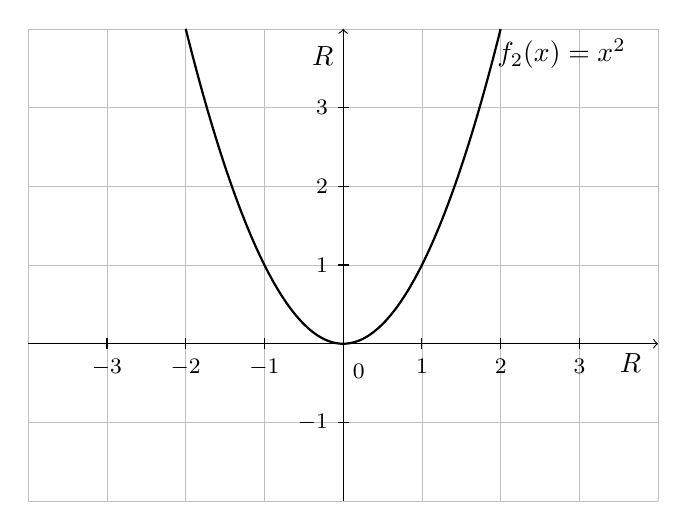
\begin{tikzpicture}
		
		% Gitternetzlinien
		\draw[xstep=1cm, ystep=1cm, very thin, color=lightgray] (-4,4) grid (4,-2);
		% x-Achse
		\draw[->] (-4,0) -- (4,0) node[below,xshift=-1em] {$\mathbb{R}$}; 
		%Zahlen auf x-Achse
		\foreach \x in {-3,...,-1}
		\draw[shift={(\x,0)},color=black] (0pt,2pt) -- (0pt,-2pt) node[below] {\footnotesize $\x$};
		\foreach \x in {1,...,3}
		\draw[shift={(\x,0)},color=black] (0pt,2pt) -- (0pt,-2pt) node[below] {\footnotesize $\x$};
		% y-Achse 
		\draw[->] (0,-2) -- (0,4) node[left,yshift=-1em] {$\mathbb{R}$};%node[above left]
		%Zahlen auf y-Achse
		\foreach \y in {-1,...,-1}
		\draw[shift={(0,\y)},color=black] (2pt,0pt) -- (-2pt,0pt) node[left] {\footnotesize $\y$};
		\foreach \y in {1,...,3}
		\draw[shift={(0,\y)},color=black] (2pt,0pt) -- (-2pt,0pt) node[left] {\footnotesize $\y$};
		%Ursprung
		\draw[color=black] (0pt,-10pt) node[right] {\footnotesize $0$};
		
		
		
		\draw[thick,color=black] plot[samples=200, domain=-2:2] 
		(\x,{\x*\x}) node[below, xshift=2.2em]{$f_2(x)=x^2$};
		
		
		
	\end{tikzpicture}\\
\end{center}
\newpage
\noindent
\textbullet  \;\;  Dies ist keine Abbildung.\\
\begin{center}
	
	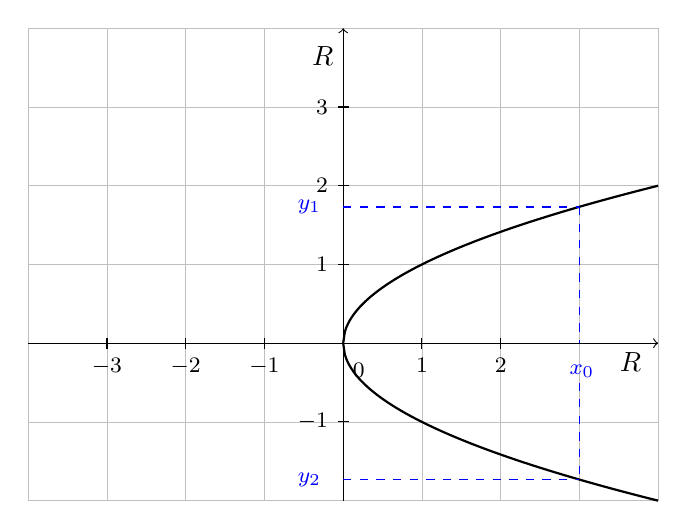
\begin{tikzpicture}
		
		% Gitternetzlinien
		\draw[xstep=1cm, ystep=1cm, very thin, color=lightgray] (-4,4) grid (4,-2);
		% x-Achse
		\draw[->] (-4,0) -- (4,0) node[below,xshift=-1em] {$\mathbb{R}$}; 
		%Zahlen auf x-Achse
		\foreach \x in {-3,...,-1}
		\draw[shift={(\x,0)},color=black] (0pt,2pt) -- (0pt,-2pt) node[below] {\footnotesize $\x$};
		\foreach \x in {1,...,2}
		\draw[shift={(\x,0)},color=black] (0pt,2pt) -- (0pt,-2pt) node[below] {\footnotesize $\x$};
		% y-Achse 
		\draw[->] (0,-2) -- (0,4) node[left,yshift=-1em] {$\mathbb{R}$};%node[above left]
		%Zahlen auf y-Achse
		\foreach \y in {-1,...,-1}
		\draw[shift={(0,\y)},color=black] (2pt,0pt) -- (-2pt,0pt) node[left] {\footnotesize $\y$};
		\foreach \y in {1,...,3}
		\draw[shift={(0,\y)},color=black] (2pt,0pt) -- (-2pt,0pt) node[left] {\footnotesize $\y$};
		%Ursprung
		\draw[color=black] (0pt,-10pt) node[right] {\footnotesize $0$};
		
		
		
		\draw[thick,color=black] plot[samples=200, domain=0:4] 
		(\x,{sqrt(\x)});
		
		\draw[thick,color=black] plot[samples=200, domain=0:4] 
		(\x,{-sqrt(\x)});
		\draw[color=blue] (-0.7,-1.73) node[right] {\footnotesize $y_2$};
		\draw[color=blue] (-0.7,1.73) node[right] {\footnotesize $y_1$};
		\draw[color=blue,dashed] (3,1.73) -- (3,0);
		\draw[color=blue,dashed] (3,-0.5) -- (3,-1.73);
		\draw[color=blue,dashed] (0,1.73) -- (3,1.73) ;
		\draw[color=blue,dashed] (0,-1.73) -- (3,-1.73);
		\draw[color=blue] (2.75,-10pt) node[right] {\footnotesize $x_0$};
	\end{tikzpicture}\\
\end{center}
Dies ist ein Widerspruch zur Definition einer Abbildung. Den Wert $x_0$ werden zwei Elemente und zwar $y_1$ und $y_2$ zugewiesen.\\
\subsection{Einschränkungen von Abbildungen}

\textbf{Definition (Einschränkung):}\\
Sei $f:\mathbb{D}_f\longmapsto \mathbb{W}_f$ eine Abbildung.\\
Die Einschränkung von $f$ auf $\mathbb{R}\subseteq \mathbb{D}_f$ ist die Abbildung.\\
\begin{center}
	$f_{|\mathbb{C}}:\mathbb{C}\longmapsto\mathbb{W}_f$ mit $f_{|\mathbb{C}}=f(x)$ für jedes $x\in\mathbb{C}$\\
\end{center}
Beispiele:\\
\textbullet$\qquad f_2:\mathbb{R}\longmapsto [0,\infty[$ mit $x\longmapsto x^2$\\
\begin{center}
	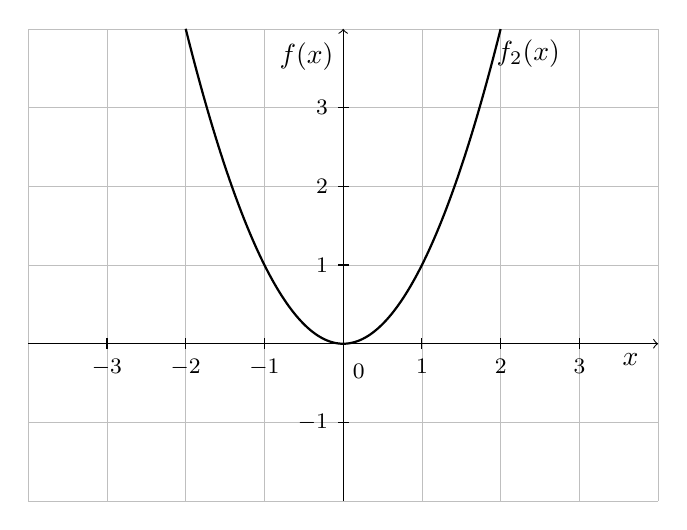
\begin{tikzpicture}
		
		% Gitternetzlinien
		\draw[xstep=1cm, ystep=1cm, very thin, color=lightgray] (-4,4) grid (4,-2);
		% x-Achse
		\draw[->] (-4,0) -- (4,0) node[below,xshift=-1em] {$x$}; 
		%Zahlen auf x-Achse
		\foreach \x in {-3,...,-1}
		\draw[shift={(\x,0)},color=black] (0pt,2pt) -- (0pt,-2pt) node[below] {\footnotesize $\x$};
		\foreach \x in {1,...,3}
		\draw[shift={(\x,0)},color=black] (0pt,2pt) -- (0pt,-2pt) node[below] {\footnotesize $\x$};
		% y-Achse 
		\draw[->] (0,-2) -- (0,4) node[left,yshift=-1em] {$f(x)$};%node[above left]
		%Zahlen auf y-Achse
		\foreach \y in {-1,...,-1}
		\draw[shift={(0,\y)},color=black] (2pt,0pt) -- (-2pt,0pt) node[left] {\footnotesize $\y$};
		\foreach \y in {1,...,3}
		\draw[shift={(0,\y)},color=black] (2pt,0pt) -- (-2pt,0pt) node[left] {\footnotesize $\y$};
		%Ursprung
		\draw[color=black] (0pt,-10pt) node[right] {\footnotesize $0$};
		
		
		
		\draw[thick,color=black] plot[samples=200, domain=-2:2] 
		(\x,{\x*\x}) node[below, xshift=1em]{$f_2(x)$};
		
		
		
	\end{tikzpicture}\\
\end{center}
\pagebreak
\textbullet $\qquad f_{2_{|[0,\infty[}}:[0,\infty[\; \longmapsto [0,\infty [\;$ mit $ x \longmapsto x^2 $\\
\begin{center}
	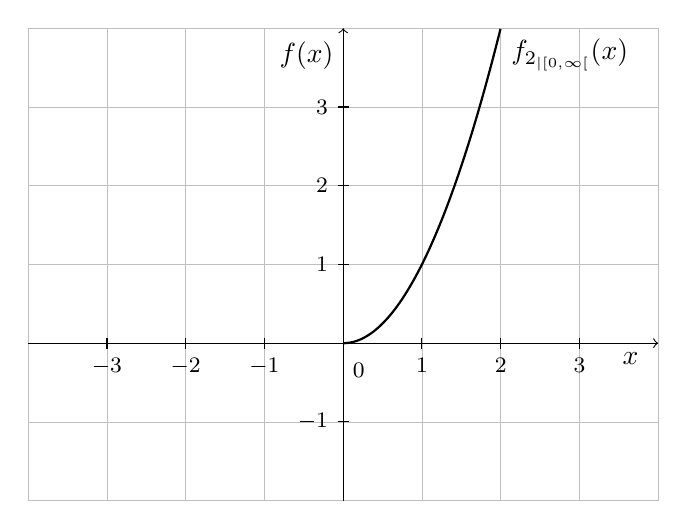
\begin{tikzpicture}
		% Gitternetzlinien
		\draw[xstep=1cm, ystep=1cm, very thin, color=lightgray] (-4,4) grid (4,-2);
		% x-Achse
		\draw[->] (-4,0) -- (4,0) node[below,xshift=-1em] {$x$}; 
		%Zahlen auf x-Achse
		\foreach \x in {-3,...,-1}
		\draw[shift={(\x,0)},color=black] (0pt,2pt) -- (0pt,-2pt) node[below] {\footnotesize $\x$};
		\foreach \x in {1,...,3}
		\draw[shift={(\x,0)},color=black] (0pt,2pt) -- (0pt,-2pt) node[below] {\footnotesize $\x$};
		% y-Achse 
		\draw[->] (0,-2) -- (0,4) node[left,yshift=-1em] {$f(x)$};%node[above left]
		%Zahlen auf y-Achse
		\foreach \y in {-1,...,-1}
		\draw[shift={(0,\y)},color=black] (2pt,0pt) -- (-2pt,0pt) node[left] {\footnotesize $\y$};
		\foreach \y in {1,...,3}
		\draw[shift={(0,\y)},color=black] (2pt,0pt) -- (-2pt,0pt) node[left] {\footnotesize $\y$};
		%Ursprung
		\draw[color=black] (0pt,-10pt) node[right] {\footnotesize $0$};
		\draw[thick,color=black] plot[samples=200, domain=0:2] 
		(\x,{\x*\x}) node[below, xshift=2.5em]{$f_{2_{|[0,\infty[}}(x)$};
		
		
		
	\end{tikzpicture}\\
\end{center}
Dies ist eine Funktion mit der Einschränkung von $f_2$ auf die Menge:$[0,\infty[$\vspace*{2mm}\\
\textbullet $\qquad f_1:\mathbb{R}\longmapsto\mathbb{R}\;$ mit $x\longmapsto 2x $\\

\begin{center}
	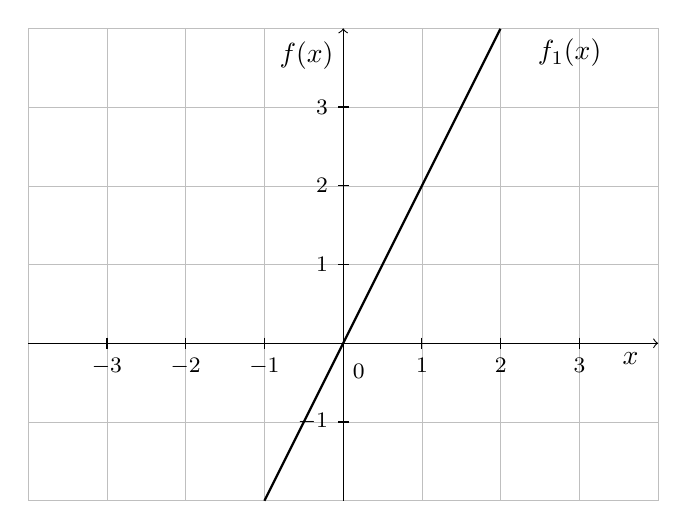
\begin{tikzpicture}
		% Gitternetzlinien
		\draw[xstep=1cm, ystep=1cm, very thin, color=lightgray] (-4,4) grid (4,-2);
		% x-Achse
		\draw[->] (-4,0) -- (4,0) node[below,xshift=-1em] {$x$}; 
		%Zahlen auf x-Achse
		\foreach \x in {-3,...,-1}
		\draw[shift={(\x,0)},color=black] (0pt,2pt) -- (0pt,-2pt) node[below] {\footnotesize $\x$};
		\foreach \x in {1,...,3}
		\draw[shift={(\x,0)},color=black] (0pt,2pt) -- (0pt,-2pt) node[below] {\footnotesize $\x$};
		% y-Achse 
		\draw[->] (0,-2) -- (0,4) node[left,yshift=-1em] {$f(x)$};%node[above left]
		%Zahlen auf y-Achse
		\foreach \y in {-1,...,-1}
		\draw[shift={(0,\y)},color=black] (2pt,0pt) -- (-2pt,0pt) node[left] {\footnotesize $\y$};
		\foreach \y in {1,...,3}
		\draw[shift={(0,\y)},color=black] (2pt,0pt) -- (-2pt,0pt) node[left] {\footnotesize $\y$};
		%Ursprung
		\draw[color=black] (0pt,-10pt) node[right] {\footnotesize $0$};
		\draw[thick,color=black] plot[samples=200, domain=-1:2] 
		(\x,{\x*2}) node[below, xshift=2.5em]{$f_1(x)$};
		
		
		
	\end{tikzpicture}\\
\end{center}
\textbullet $\qquad f_{1_{|\mathbb{Z}}}:\mathbb{Z}\longmapsto\mathbb{Z}\;$ mit $x\longmapsto 2x $$\qquad$ Bemerkung: ($\longmapsto\mathbb{Z}$, weil $2\cdot x$ immer $\in\mathbb{Z}$ ist)\\

\begin{center}
	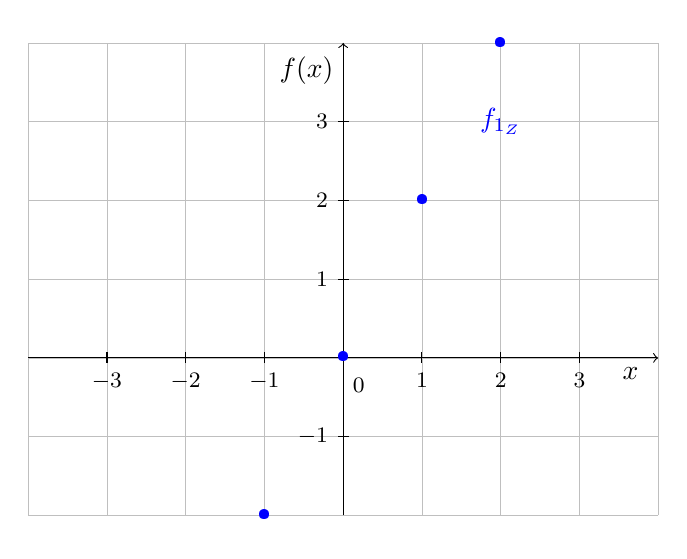
\begin{tikzpicture}
		% Gitternetzlinien
		\draw[xstep=1cm, ystep=1cm, very thin, color=lightgray] (-4,4) grid (4,-2);
		% x-Achse
		\draw[->] (-4,0) -- (4,0) node[below,xshift=-1em] {$x$}; 
		%Zahlen auf x-Achse
		\foreach \x in {-3,...,-1}
		\draw[shift={(\x,0)},color=black] (0pt,2pt) -- (0pt,-2pt) node[below] {\footnotesize $\x$};
		\foreach \x in {1,...,3}
		\draw[shift={(\x,0)},color=black] (0pt,2pt) -- (0pt,-2pt) node[below] {\footnotesize $\x$};
		% y-Achse 
		\draw[->] (0,-2) -- (0,4) node[left,yshift=-1em] {$f(x)$};%node[above left]
		%Zahlen auf y-Achse
		\foreach \y in {-1,...,-1}
		\draw[shift={(0,\y)},color=black] (2pt,0pt) -- (-2pt,0pt) node[left] {\footnotesize $\y$};
		\foreach \y in {1,...,3}
		\draw[shift={(0,\y)},color=black] (2pt,0pt) -- (-2pt,0pt) node[left] {\footnotesize $\y$};
		%Ursprung
		\draw[color=black] (0pt,-10pt) node[right] {\footnotesize $0$};
		
		
		\draw[color=blue] (1,2) node {\textbullet};
		\draw[color=blue] (2,4) node {\textbullet};
		\draw[color=blue] (0,0) node {\textbullet};
		\draw[color=blue] (-1,-2) node {\textbullet};
		\draw[color=blue] (2,3) node {$f_{1_{\lvert\mathbb{Z}}}$};
		
	\end{tikzpicture}\\
\end{center}
\pagebreak
\subsection{Bild einer Abbildungen}

\textbf{Definition (Bild):}\\
Sei $f:\mathbb{D}_f\longmapsto\mathbb{W}_f$ eine Abbildung.\\
Das Bild von $f$ ist die Menge:\\
\begin{align*}
	\mathrm{Bild}(f)=f(\mathbb{D}_f)=\{f(x) | x\in\mathbb{D}_f  \}
\end{align*}
Beispiele:\\
\textbullet$\qquad f_2:\mathbb{R}\longmapsto [0,\infty[ \qquad$ mit $x\longmapsto x^2$\\
\begin{center}
	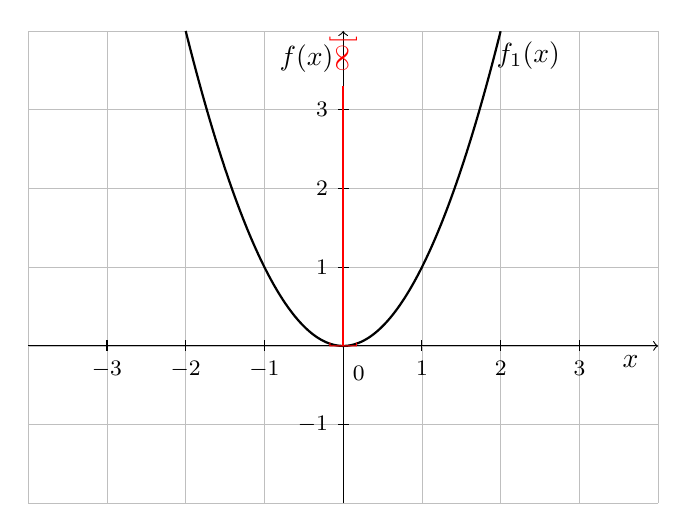
\begin{tikzpicture}
		
		% Gitternetzlinien
		\draw[xstep=1cm, ystep=1cm, very thin, color=lightgray] (-4,4) grid (4,-2);
		% x-Achse
		\draw[->] (-4,0) -- (4,0) node[below,xshift=-1em] {$x$}; 
		%Zahlen auf x-Achse
		\foreach \x in {-3,...,-1}
		\draw[shift={(\x,0)},color=black] (0pt,2pt) -- (0pt,-2pt) node[below] {\footnotesize $\x$};
		\foreach \x in {1,...,3}
		\draw[shift={(\x,0)},color=black] (0pt,2pt) -- (0pt,-2pt) node[below] {\footnotesize $\x$};
		% y-Achse 
		\draw[->] (0,-2) -- (0,4) node[left,yshift=-1em] {$f(x)$};%node[above left]
		%Zahlen auf y-Achse
		\foreach \y in {-1,...,-1}
		\draw[shift={(0,\y)},color=black] (2pt,0pt) -- (-2pt,0pt) node[left] {\footnotesize $\y$};
		\foreach \y in {1,...,3}
		\draw[shift={(0,\y)},color=black] (2pt,0pt) -- (-2pt,0pt) node[left] {\footnotesize $\y$};
		%Ursprung
		\draw[color=black] (0pt,-10pt) node[right] {\footnotesize $0$};
		
		
		
		\draw[thick,color=black] plot[samples=200, domain=-2:2] 
		(\x,{\x*\x}) node[below, xshift=1em]{$f_1(x)$};
		\draw[thick,color=red] (0,3.7) node[rotate=-90] {$]\infty$};
		\draw[thick,color=red] (0,0) node[rotate=-90] {$]$};
		\draw[thick,color=red] (0,0) -- (0,3.3); 
	\end{tikzpicture}\\
\end{center}
\begin{align*}
	\mathrm{Bild}_{(f_{2})}=\textcolor{red}{[0,\infty[}=\mathbb{W}_f
\end{align*}
\textbullet $\qquad$Bestimme das $ \mathrm{Bild}_{\big(f_{2_{|[0,4]}}\big)}\; $von der Funktion: $ f_{2_{|[2,4]}}$.\\
\begin{center}
	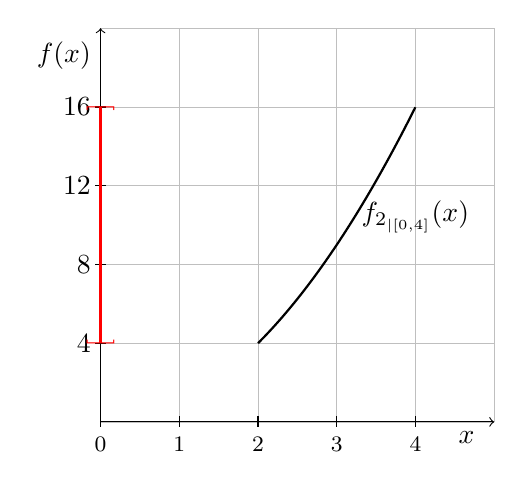
\begin{tikzpicture}
		yscale=<0.2>;
		% Gitternetzlinien
		\draw[xstep=1cm, ystep=1cm, very thin, color=lightgray] (0,5) grid (5,0);
		% x-Achse
		\draw[->] (0,0) -- (5,0) node[below,xshift=-1em] {$x$}; 
		%Zahlen auf x-Achse
		%\foreach \x in {0,...,4}
		%\draw[shift={(\x,0)},color=black] (0pt,2pt) -- (0pt,-2pt) node[below] {\footnotesize $\x$};
		\foreach \x in {0,...,4}
		\draw[shift={(\x,0)},color=black] (0pt,2pt) -- (0pt,-2pt) node[below] {\footnotesize $\x$};
		% y-Achse 
		
		\draw[->] (0,0) -- (0,5) node[left,yshift=-1em] {$f(x)$};%node[above left]
		%Zahlen auf y-Achse
		%\foreach \y in {1,...,4}
		%\draw[shift={(0,\y)},color=black] (2pt,0pt) -- (-2pt,0pt) node[left] {\footnotesize $\y$};
		\foreach \y in {1,...,4}
		\draw[shift={(0,\y)},color=black,] (2pt,0pt) -- (-2pt,0pt) node[left] {\footnotesize };
		\draw[thick,color=black,yscale=0.25] plot[samples=200, domain=2:4] 
		(\x,{\x*\x}) node[below,yshift=-3em]{$f_{2_{|[0,4]}}(x)$};
		\draw[color=black] (0,1) node[left] {$4$};
		\draw[color=black] (0,2) node[left] {$8$};
		\draw[color=black] (0,3) node[left] {$12$};
		\draw[color=black] (0,4) node[left] {$16$};
		\draw[thick,color=red] (0,1) node[rotate=-90] {$]$};
		\draw[thick,color=red] (0,4) node[rotate=-90] {$[$};
		\draw[thick,color=red] (0,1) -- (0,4); 
	\end{tikzpicture}\\
\end{center}
\begin{align*}
	\mathrm{Bild}_{(f_{2_{[2,4]}})}=[4,16]\\
\end{align*}
\newpage
\noindent
\textbullet $\qquad$Bestimme das $  \mathrm{Bild}_{\big (f_{2_{|\{5\}}}\big )}\; $von der Funktion: $ f_{2_{|\{5\}}}$.\\
\begin{center}
	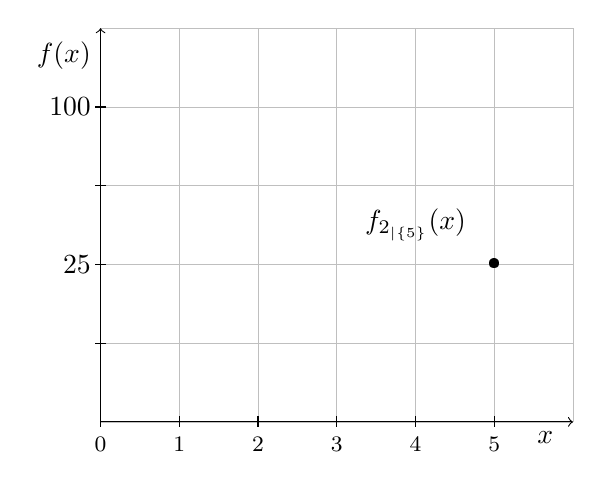
\begin{tikzpicture}
		yscale=<0.2>;
		% Gitternetzlinien
		\draw[xstep=1cm, ystep=1cm, very thin, color=lightgray] (0,5) grid (6,0);
		% x-Achse
		\draw[->] (0,0) -- (6,0) node[below,xshift=-1em] {$x$}; 
		%Zahlen auf x-Achse
		%\foreach \x in {0,...,6}
		%\draw[shift={(\x,0)},color=black] (0pt,2pt) -- (0pt,-2pt) node[below] {\footnotesize $\x$};
		\foreach \x in {0,...,5}
		\draw[shift={(\x,0)},color=black] (0pt,2pt) -- (0pt,-2pt) node[below] {\footnotesize $\x$};
		% y-Achse 
		
		\draw[->] (0,0) -- (0,5) node[left,yshift=-1em] {$f(x)$};%node[above left]
		%Zahlen auf y-Achse
		%\foreach \y in {1,...,4}
		%\draw[shift={(0,\y)},color=black] (2pt,0pt) -- (-2pt,0pt) node[left] {\footnotesize $\y$};
		\foreach \y in {1,...,4}
		\draw[shift={(0,\y)},color=black,] (2pt,0pt) -- (-2pt,0pt) node[left] {\footnotesize };
		
		\draw[color=black] (5,2) node {\textbullet};
		\draw[color=black] (0,2) node[left] {$25$};
		%\draw[color=black] (0,3) node[left] {$12$};
		\draw[color=black] (0,4) node[left] {$100$};
		\draw[color=black] (4,2.5) node {$f_{2_{|\{5\}}}(x)$};
		
	\end{tikzpicture}\\
\end{center}
\begin{align*}
	\mathrm{Bild}_{\big (f_{2_{|\{5\}}}\big )}\;=\;\{25\}
\end{align*}
\subsection{Urbild von Abbildungen}

\textbf{Definition (Urbild):}\\
Das Urbild von $\mathbb{V}\subseteq \mathbb{W}_f$ unter $f$ ist die Menge:\\
\begin{align*}
	f^{-1}(\mathbb{V})=\{ x\in\mathbb{D}_f\;|\;f(x)\in\mathbb{V}\}\subseteq\mathbb{D}_f
\end{align*}
Achtung: $f^{-1}$ ist nicht die Umkehrfunktion !!\\
\begin{center}
	
	
	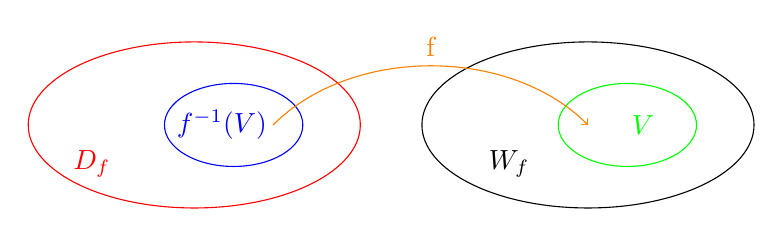
\begin{tikzpicture} 
		\draw[color=black] (5,0) ellipse (60pt and 30pt); 
		\draw[color=red] (0,0) ellipse (60pt and 30pt);
		\draw[color=blue] (0.5,0) ellipse (25pt and 15pt);
		\draw[color=green] (5.5,0) ellipse (25pt and 15pt);
		
		\draw[color=black] (4,-.5) node { $\mathbb{W}_f$};
		\draw[color=red] (-1.3,-.5) node { $\mathbb{D}_f$};
		\draw[color=blue] (0.35,0) node { $f^{-1}(\mathbb{V})$};
		\draw[color=green] (5.7,0) node { $\mathbb{V}$};
		
		\draw[->,orange] (1, 0) .. controls(2, 1) and(4,1) .. node[above,sloped] {f}(5, 0);
	\end{tikzpicture}
	
\end{center}
Beispiel:\\
$f_2 :\mathbb{R}\longmapsto[0,\infty[$ mit $x\longmapsto x^2$\\

\textbullet\;\; Bestimme das Urbild von: $f^{-1}_{2_{([0,\infty[)}}$



\begin{center}
	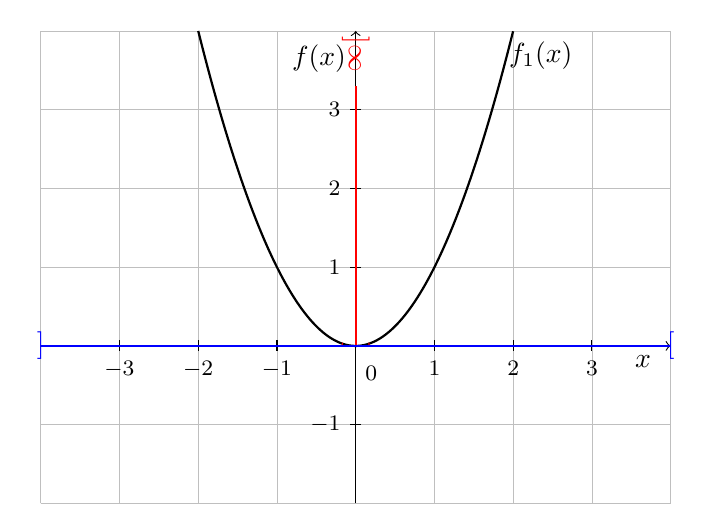
\begin{tikzpicture}
		
		% Gitternetzlinien
		\draw[xstep=1cm, ystep=1cm, very thin, color=lightgray] (-4,4) grid (4,-2);
		% x-Achse
		\draw[->] (-4,0) -- (4,0) node[below,xshift=-1em] {$x$}; 
		%Zahlen auf x-Achse
		\foreach \x in {-3,...,-1}
		\draw[shift={(\x,0)},color=black] (0pt,2pt) -- (0pt,-2pt) node[below] {\footnotesize $\x$};
		\foreach \x in {1,...,3}
		\draw[shift={(\x,0)},color=black] (0pt,2pt) -- (0pt,-2pt) node[below] {\footnotesize $\x$};
		% y-Achse 
		\draw[->] (0,-2) -- (0,4) node[left,yshift=-1em] {$f(x)$};%node[above left]
		%Zahlen auf y-Achse
		\foreach \y in {-1,...,-1}
		\draw[shift={(0,\y)},color=black] (2pt,0pt) -- (-2pt,0pt) node[left] {\footnotesize $\y$};
		\foreach \y in {1,...,3}
		\draw[shift={(0,\y)},color=black] (2pt,0pt) -- (-2pt,0pt) node[left] {\footnotesize $\y$};
		%Ursprung
		\draw[color=black] (0pt,-10pt) node[right] {\footnotesize $0$};
		
		
		
		\draw[thick,color=black] plot[samples=200, domain=-2:2] 
		(\x,{\x*\x}) node[below, xshift=1em]{$f_1(x)$};
		\draw[thick,color=red] (0,3.7) node[rotate=-90] {$]\infty$};
		\draw[thick,color=red] (0,0) node[rotate=-90] {$]$};
		\draw[thick,color=red] (0,0) -- (0,3.3); 
		\draw[color=blue,thick] (-4,0) -- (4,0) node {$[$};
		\draw[color=blue,thick] (-4,0) node {$]$}; 
	\end{tikzpicture}\\
	
\end{center}
\begin{align*}
	f^{-1}_{2_{(\textcolor{red}{[0,\infty[})}}=\textcolor{blue}{\mathbb{R}}
\end{align*}

\textbullet\;\; Bestimme das Urbild von: $f^{-1}_{2_{([2,4])}}$
\begin{center}
	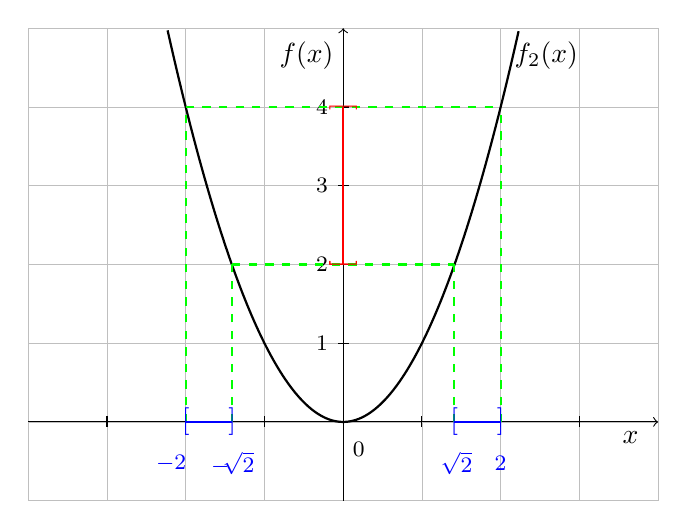
\begin{tikzpicture}
		
		% Gitternetzlinien
		\draw[xstep=1cm, ystep=1cm, very thin, color=lightgray] (-4,5) grid (4,-1);
		% x-Achse
		\draw[->] (-4,0) -- (4,0) node[below,xshift=-1em] {$x$}; 
		%Zahlen auf x-Achse
		\foreach \x in {-3,...,-1}
		\draw[shift={(\x,0)},color=black] (0pt,2pt) -- (0pt,-2pt);
		\foreach \x in {1,...,3}
		\draw[shift={(\x,0)},color=black] (0pt,2pt) -- (0pt,-2pt);
		\draw[color=blue] (-1.8,-15pt) node[right] {\footnotesize $- \sqrt[]{2}$};
		\draw[color=blue] (-2.5,-15pt) node[right] {\footnotesize $-2$};
		\draw[color=blue] (1.2,-15pt) node[right] {\footnotesize $ \sqrt[]{2}$};
		\draw[color=blue] (1.8,-15pt) node[right] {\footnotesize $2$};
		% y-Achse 
		\draw[->] (0,-1) -- (0,5) node[left,yshift=-1em] {$f(x)$};%node[above left]
		%Zahlen auf y-Achse
		%\foreach \y in {0,...,-1}
		%\draw[shift={(0,\y)},color=black] (2pt,0pt) -- (-2pt,0pt) node[left] {\footnotesize $\y$};
		\foreach \y in {1,...,4}
		\draw[shift={(0,\y)},color=black] (2pt,0pt) -- (-2pt,0pt) node[left] {\footnotesize $\y$};
		%Ursprung
		\draw[color=black] (0pt,-10pt) node[right] {\footnotesize $0$};
		
		
		
		\draw[thick,color=black] plot[samples=200, domain=-2.23:2.23] 
		(\x,{\x*\x}) node[below, xshift=1em]{$f_2(x)$};
		\draw[color=green,dashed,thick] (-2,4) -- (2,4);
		\draw[color=green,dashed,thick] (-2,0) -- (-2,4);
		\draw[color=green,dashed,thick] (2,0) -- (2,4);
		\draw[color=red,thick] (0,2)node[rotate=90] {[} -- (0,4);
		\draw[color=green,dashed,thick] (-1.41,2) -- (1.41,2);
		\draw[color=green,dashed,thick] (-1.41,0) -- (-1.41,2);
		\draw[color=green,dashed,thick] (1.41,0) -- (1.41,2);
		\draw[color=blue,thick] (-2,0)node{[} -- (-1.41,0)node{]};
		\draw[color=blue,thick] (1.41,0)node{[} -- (2,0)node{]};
		\draw[color=red,thick] (0,2)node[rotate=90] {[} -- (0,4)node[rotate=90] {]};
		
	\end{tikzpicture}\\
\end{center}
\begin{align*}
	f^{-1}_{2_{(\textcolor{red}{[2,4]})}}=\textcolor{blue}{[-2,-\sqrt{2}]\cup[\sqrt{2},2]}
\end{align*}
\textbullet\;\; Bestimme das Urbild von: $f^{-1}_{2_{(\{9\})}}$
\begin{center}
	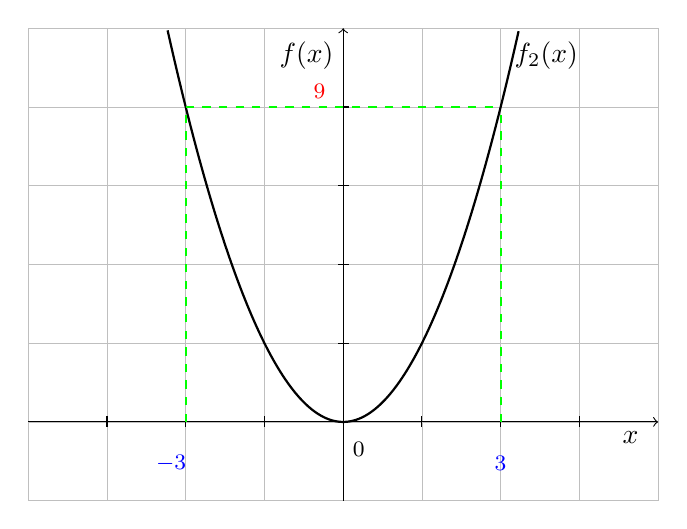
\begin{tikzpicture}
		
		% Gitternetzlinien
		\draw[xstep=1cm, ystep=1cm, very thin, color=lightgray] (-4,5) grid (4,-1);
		% x-Achse
		\draw[->] (-4,0) -- (4,0) node[below,xshift=-1em] {$x$}; 
		%Zahlen auf x-Achse
		\foreach \x in {-3,...,-1}
		\draw[shift={(\x,0)},color=black] (0pt,2pt) -- (0pt,-2pt);
		\foreach \x in {1,...,3}
		\draw[shift={(\x,0)},color=black] (0pt,2pt) -- (0pt,-2pt);
		
		\draw[color=blue] (-2.5,-15pt) node[right] {\footnotesize $-3$};
		
		\draw[color=blue] (1.8,-15pt) node[right] {\footnotesize $3$};
		% y-Achse 
		\draw[->] (0,-1) -- (0,5) node[left,yshift=-1em] {$f(x)$};%node[above left]
		%Zahlen auf y-Achse
		\foreach \y in {0,...,4}
		\draw[shift={(0,\y)},color=black] (2pt,0pt) -- (-2pt,0pt);
		
		
		\draw[color=black] (0pt,-10pt) node[right] {\footnotesize $0$};
		
		\draw[color=red] (-0.5,4.2) node[right] {\footnotesize $9$};
		
		\draw[thick,color=black] plot[samples=200, domain=-2.23:2.23] 
		(\x,{\x*\x}) node[below, xshift=1em]{$f_2(x)$};
		\draw[color=green,dashed,thick] (-2,4) -- (2,4);
		\draw[color=green,dashed,thick] (-2,0) -- (-2,4);
		\draw[color=green,dashed,thick] (2,0) -- (2,4);
		
		%\draw[color=green,dashed,thick] (-1.41,2) -- (1.41,2);
		%\draw[color=green,dashed,thick] (-1.41,0) -- (-1.41,2);
		%\draw[color=green,dashed,thick] (1.41,0) -- (1.41,2);
		
		
		
	\end{tikzpicture}\\
\end{center}
\begin{align*}
	f^{-1}_{2_{(\textcolor{red}{\{9\}})}}=\textcolor{blue}{\{-3,3\}}
\end{align*}
\subsection{Aufgabe zum Thema Bild und Urbild}

Sei $f:\mathbb{R}\longmapsto \mathbb{R}$ mit $f(x)=2x^2-2$ gegeben.\vspace*{2mm}\\
\begin{tabular}[t]{lll}% l=linksbündig r=rechtsbündig
	(i) & Bestimme $\mathrm{Bild}(f)$.  \\
	(ii) & Berechne $f^{-1}([6,30])$. \\
	(iii)&Berechne $f^{-1}(\{\frac{23}{7}\})$.\\	
\end{tabular} \vspace*{2mm}\\
zu (i):
\begin{quote}
	$\mathrm{Bild}(f)=?$\\
	Im positiven Bereich, wenn man große x-Werte in $f(x)$ einsetzt laufen die Werte in das Unendliche $\Rightarrow\infty [ $ .\\
	Die Funktion kann nicht kleiner als -2 werden $\Rightarrow [-2$ .\\
	\begin{align*}
		\mathrm{Bild}(f)=[-2,\infty[
	\end{align*}
\end{quote}
\begin{center}
	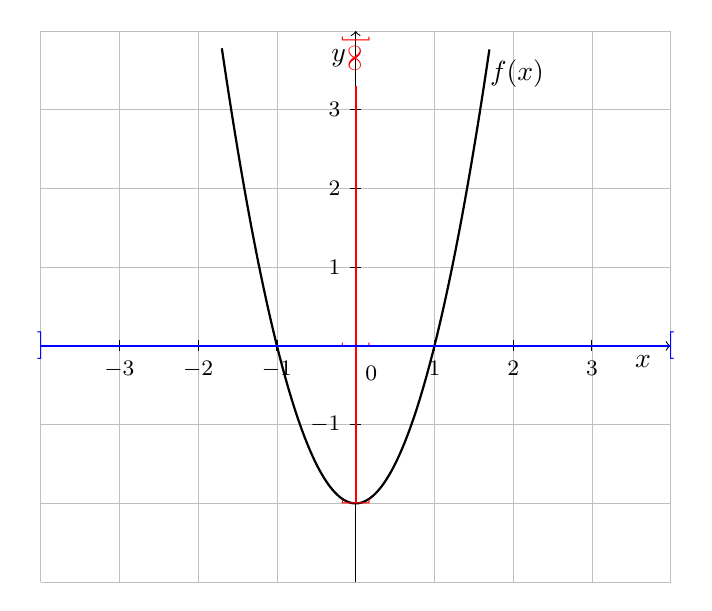
\begin{tikzpicture}
		
		% Gitternetzlinien
		\draw[xstep=1cm, ystep=1cm, very thin, color=lightgray] (-4,4) grid (4,-3);
		% x-Achse
		\draw[->] (-4,0) -- (4,0) node[below,xshift=-1em] {$x$}; 
		%Zahlen auf x-Achse
		\foreach \x in {-3,...,-1}
		\draw[shift={(\x,0)},color=black] (0pt,2pt) -- (0pt,-2pt) node[below] {\footnotesize $\x$};
		\foreach \x in {1,...,3}
		\draw[shift={(\x,0)},color=black] (0pt,2pt) -- (0pt,-2pt) node[below] {\footnotesize $\x$};
		% y-Achse 
		\draw[->] (0,-3) -- (0,4) node[left,yshift=-1em] {$y$};%node[above left]
		%Zahlen auf y-Achse
		\foreach \y in {-1,...,-1}
		\draw[shift={(0,\y)},color=black] (2pt,0pt) -- (-2pt,0pt) node[left] {\footnotesize $\y$};
		\foreach \y in {1,...,3}
		\draw[shift={(0,\y)},color=black] (2pt,0pt) -- (-2pt,0pt) node[left] {\footnotesize $\y$};
		%Ursprung
		\draw[color=black] (0pt,-10pt) node[right] {\footnotesize $0$};
		
		
		
		\draw[thick,color=black] plot[samples=200, domain=-1.7:1.7] 
		(\x,{2*\x*\x-2}) node[below, xshift=1em]{$f(x)$};
		\draw[thick,color=red] (0,3.7) node[rotate=-90] {$]\infty$};
		\draw[thick,color=red] (0,0) node[rotate=-90] {$]$};
		\draw[thick,color=red] (0,-2) node[rotate=-90] {$]$}-- (0,3.3); 
		\draw[color=blue,thick] (-4,0) -- (4,0) node {$[$};
		\draw[color=blue,thick] (-4,0) node {$]$}; 
	\end{tikzpicture}\\
	
	
\end{center}
zu (ii):
\begin{quote}
	Bestimme Urbild von: $f^{-1}({[6,30]})$\vspace*{2mm}\\
	Nr: Berechnung der Intervallgrenzen:\\
	$\blacktriangleright \quad f(x)=6\Leftrightarrow 2x^2-2=6\Leftrightarrow 2x^2=8\Leftrightarrow x^2=4 \Rightarrow x_{1,2}=\pm 2 $\\
	$\blacktriangleright \quad f(x)=30\Leftrightarrow2x^2-2=30\Leftrightarrow x^2=16\Rightarrow x_{1,2}=\pm 4$\\
	\begin{align*}
		f^{-1}([6,30])=[-4,-2]\cup [2,4]
	\end{align*}
\end{quote}
\begin{center}
	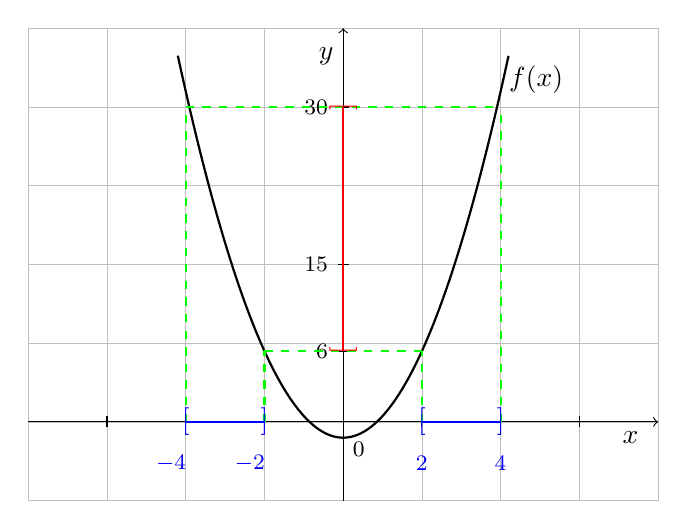
\begin{tikzpicture}
		
		% Gitternetzlinien
		\draw[xstep=1cm, ystep=1cm, very thin, color=lightgray] (-4,5) grid (4,-1);
		% x-Achse
		\draw[->] (-4,0) -- (4,0) node[below,xshift=-1em] {$x$}; 
		%Zahlen auf x-Achse
		\foreach \x in {-3,...,-1}
		\draw[shift={(\x,0)},color=black] (0pt,2pt) -- (0pt,-2pt);
		\foreach \x in {1,...,3}
		\draw[shift={(\x,0)},color=black] (0pt,2pt) -- (0pt,-2pt);
		\draw[color=blue] (-1.5,-15pt) node[right] {\footnotesize $-2$};
		\draw[color=blue] (-2.5,-15pt) node[right] {\footnotesize $-4$};
		\draw[color=blue] (0.8,-15pt) node[right] {\footnotesize $2$};
		\draw[color=blue] (1.8,-15pt) node[right] {\footnotesize $4$};
		% y-Achse 
		\draw[->] (0,-1) -- (0,5) node[left,yshift=-1em] {$y$};%node[above left]
		
		%Zahlen auf y-Achse
		%\foreach \y in {0,...,-1}
		%\draw[shift={(0,\y)},color=black] (2pt,0pt) -- (-2pt,0pt) node[left] {\footnotesize $\y$};
		
		\draw[shift={(0,0.9)},color=black] (2pt,0pt) -- (-2pt,0pt) node[left] {\footnotesize $6$};
		\draw[shift={(0,2)},color=black] (2pt,0pt) -- (-2pt,0pt) node[left] {\footnotesize $15$};
		%\draw[shift={(0,3)},color=black] (2pt,0pt) -- (-2pt,0pt) node[left] {\footnotesize $30$};
		\draw[shift={(0,4)},color=black] (2pt,0pt) -- (-2pt,0pt) node[left] {\footnotesize $30$};
		%Ursprung
		\draw[color=black] (0pt,-10pt) node[right] {\footnotesize $0$};
		
		
		
		\draw[thick,color=black] plot[samples=200, domain=-2.1:2.1] 
		(\x,{1.1*\x*\x-0.2}) node[below, xshift=1em]{$f(x)$};
		\draw[color=green,dashed,thick] (-2,4) -- (2,4);
		\draw[color=green,dashed,thick] (-2,0) -- (-2,4);
		\draw[color=green,dashed,thick] (2,0) -- (2,4);
		%\draw[color=red,thick] (0,0)node[rotate=90] {[} -- (0,4);
		\draw[color=green,dashed,thick] (-1,0.9) -- (1,0.9);
		\draw[color=green,dashed,thick] (-1,0) -- (-1,0.9);
		\draw[color=green,dashed,thick] (1,0) -- (1,0.9);
		\draw[color=blue,thick] (-2,0)node{[} -- (-1,0)node{]};
		\draw[color=blue,thick] (1,0)node{[} -- (2,0)node{]};
		\draw[color=red,thick] (0,0.9)node[rotate=90] {[} -- (0,4)node[rotate=90] {]};
		
	\end{tikzpicture}\\
\end{center}
zu (iii):\\
\begin{quote}
	Bestimme Urbild von: $f^{-1}(\{\frac{23}{7}\})$\vspace*{2mm}\\
	Nr: Berechnung des Urbildes:\\
	$\blacktriangleright\quad f(x)=\frac{23}{7}	\Leftrightarrow 2x^2-2=\frac{23}{7}\Leftrightarrow 2x^2=\frac{23}{7}+2=\frac{37}{7}\Leftrightarrow x^2=\frac{37}{14}\Rightarrow x_{1,2}=\pm \sqrt{\smash[b]{\scriptscriptstyle\frac{37}{14}}}$\\
	\begin{align*}
		f^{-1}(\{\tfrac{23}{7}\})=\{ -\sqrt{\scriptscriptstyle\frac{37}{14}},\sqrt{\scriptscriptstyle\frac{37}{14}}\}
	\end{align*}
\end{quote}
\begin{center}
	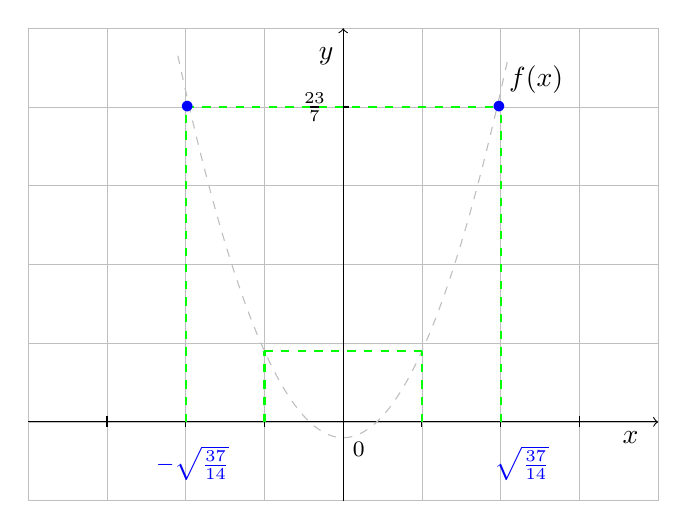
\begin{tikzpicture}
		
		% Gitternetzlinien
		\draw[xstep=1cm, ystep=1cm, very thin, color=lightgray] (-4,5) grid (4,-1);
		% x-Achse
		\draw[->] (-4,0) -- (4,0) node[below,xshift=-1em] {$x$}; 
		%Zahlen auf x-Achse
		\foreach \x in {-3,...,-1}
		\draw[shift={(\x,0)},color=black] (0pt,2pt) -- (0pt,-2pt);
		\foreach \x in {1,...,3}
		\draw[shift={(\x,0)},color=black] (0pt,2pt) -- (0pt,-2pt);
		%\draw[color=blue] (-1.5,-15pt) node[right] {\footnotesize $-2$};
		\draw[color=blue] (-2.5,-15pt) node[right] {\footnotesize $-\sqrt{\frac{37}{14}}$};
		%draw[color=blue] (0.8,-15pt) node[right] {\footnotesize $\sqrt{\frac{37}{14}}$};
		\draw[color=blue] (1.8,-15pt) node[right] {\footnotesize $\sqrt{\frac{37}{14}}$};
		% y-Achse 
		\draw[->] (0,-1) -- (0,5) node[left,yshift=-1em] {$y$};%node[above left]
		
		%Zahlen auf y-Achse
		%\foreach \y in {0,...,-1}
		%\draw[shift={(0,\y)},color=black] (2pt,0pt) -- (-2pt,0pt) node[left] {\footnotesize $\y$};
		
		%\draw[shift={(0,0.9)},color=black] (2pt,0pt) -- (-2pt,0pt) node[left] {\footnotesize $6$};
		%\draw[shift={(0,2)},color=black] (2pt,0pt) -- (-2pt,0pt) node[left] {\footnotesize $15$};
		%\draw[shift={(0,3)},color=black] (2pt,0pt) -- (-2pt,0pt) node[left] {\footnotesize $30$};
		\draw[shift={(0,4)},color=black] (2pt,0pt) -- (-2pt,0pt) node[left] {\footnotesize $\frac{23}{7}$};
		%Ursprung
		\draw[color=black] (0pt,-10pt) node[right] {\footnotesize $0$};
		
		
		
		\draw[dashed,color=lightgray] plot[samples=200, domain=-2.1:2.1] 
		(\x,{1.1*\x*\x-0.2}) node[below, xshift=1em]{$\textcolor{black}{f(x)}$};
		\draw[color=green,dashed,thick] (-2,4) -- (2,4);
		\draw[color=green,dashed,thick] (-2,0) -- (-2,4);
		\draw[color=green,dashed,thick] (2,0) -- (2,4);
		%\draw[color=red,thick] (0,0)node[rotate=90] {[} -- (0,4);
		\draw[color=green,dashed,thick] (-1,0.9) -- (1,0.9);
		\draw[color=green,dashed,thick] (-1,0) -- (-1,0.9);
		\draw[color=green,dashed,thick] (1,0) -- (1,0.9);
		%\draw[color=blue,thick] (-2,0)node{[} -- (-1,0)node{]};
		%\draw[color=blue,thick] (1,0)node{[} -- (2,0)node{]};
		%\draw[color=red,thick] (0,0.9)node[rotate=90] {[} -- (0,4)node[rotate=90] {]};
		\draw[color=blue,thick](1.98,4) node {$\bullet$};
		\draw[color=blue,thick](-1.98,4) node {$\bullet$};
	\end{tikzpicture}\\
\end{center}